\documentclass[a4paper,11pt]{article}

\usepackage[plain]{fullpage} %Error.
\usepackage{graphicx}  %This enables the inclusion of pdf graphic files in figures
\usepackage{wrapfig}
\usepackage{array}
\usepackage[hidelinks]{hyperref}
\usepackage{color}
\definecolor{light-gray}{gray}{0.95}
\usepackage{listings}
\lstset{
basicstyle=\scriptsize, 
morecomment=[l]{/*},
backgroundcolor=\color{light-gray}, 
xleftmargin=.10in,
xrightmargin=.10in,
language=C
}

\title{\textbf{Report: Assignment 3}}
\author{Group 9: \O yvin Richardsen, Sandor Zeestraten, Stian Habbestad}
\date{{Norwegian University of Science and Technology \\
TDT4258 Energy Efficient Computer Design \\}
\today}

\begin{document}
\maketitle

\begin{abstract}
In this assignment we write C code for an AVR microcontroller on linux. The goal is to make a game be played on the development board. Through this assignment we aim to become more familiar with C coding for AVR32, linux and how to write a driver for linux. 
\end{abstract}

\bigskip
\tableofcontents
\newpage

\section{Introduction}

In this exercise we write a game in C, which is executed on top of linux on a STK1000 development board. We have written a pair of drivers to handle leds and buttons...................

\section{Description and methodology}

\textbf{Forrige rapport: organize report better (overview and block diagram before description of code fragments and functions). Ergo, block diagram her?}\\

First off we started out with trying to install linux on the STK1000 development board. This turned out to be a tricky affair. We had a step by step guide for compiling linux that we followed, but with no luck. Luckily there was mentioned an image of a precompiled linux that we could extract to the SD card. After some mixing back and forth with environment variables from the other u-boot.bin file(from itslearning) into the one we were using we finally started to get somewhere. Another group posted a guide on itslearning that worked for us.

Once we had linux up and running we started out with a simple "Hello world" program to verify things were working. Now we started out with programming a driver for the LEDs. We sometimes thought we had found the solution, but we still hadn't figured it out correctly. We gave the LED driver a pause and started to communicate with the frame buffer in linux. 

First off we thought maybe this file had to be a kernel module as well, but we soon understood that we needed acceess to quite a few libraries to make the memory mapping work. We started with generating a random bit values for the display and went on with more logical values, for example a third of the screen was made red. As we tried to read bit values from an image of the file format bitmap, we started to see that there were some errors in regards to how we read the file. 

\emph{linux compiling, image to sd, previous assignment, driver(led and button), framebuffer, porting of sokoban to C, sound, generated sounds, }

\subsection{Game}
\begin{figure}
\centering
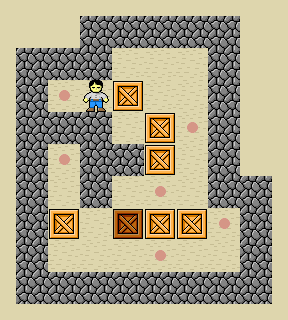
\includegraphics{images/sokoban.png}
\caption{A screenshot of another implementation of Sokoban by Borgar Porsteinsson \cite{sokobanscreen}.}
\label{fig:sokobanimage}
\end{figure}

\subsubsection{Sokoban}
The game we chose to implement was a simple top-down puzzle game called \textit{Sokoban}\cite{sokoban}. The point of the game is for the player to push boxes onto marked goal squares. The levels are small maps confined by walls which cannot be walked through. The puzzle is solved when all the boxes are on the goal squares. We had some previous experience of implementing this game in Java in the course TDT4100: Object Oriented Programming. We therefore chose to port it to C. See figure~\ref{fig:sokobanimage} for a screenshot of another implementation of Sokoban.

\subsubsection{Levels}
The levels are defined by it's dimensions and an array of characters of the different elements. For more information see the level format page on Sokoban Wiki \cite{sokobanlevel}. See table \ref{tab:levelformat} for the level format we use. The first level is defined in figure \ref{fig:leveldef} and is the simplest solvable level. The only move available is to push the box to the left.

\begin{table}
\centering
\begin{tabular}{|l|l|}
\hline \textbf{Level element} & \textbf{Character} \\ 
\hline Wall & \# \\ 
\hline Player & @ \\ 
\hline Player on goal square & + \\ 
\hline Box & \$ \\ 
\hline Box on goal square & * \\ 
\hline Goal square & . \\ 
\hline Floor & (whitespace) \\ 
\hline 
\end{tabular}
\caption{The level format.}
\label{tab:levelformat}
\end{table}

\begin{figure}
\begin{lstlisting}
// From sokoban_leveldefs.h
#define level1dimX 5
#define level1dimY 3
char level1[] = "######@$.######";

// The level above looks like this when formatted.
#####
#@$.#
#####
\end{lstlisting}
\caption{Definition of the first level.}
\label{fig:leveldef}
\end{figure}

\subsubsection{Controls}
The controls of the game are listed in table~\ref{tab:gamecontrols}. 
\begin{table}
\centering
\begin{tabular}{|l|l|}
\hline \textbf{Switch} & \textbf{Action} \\ 
\hline SW7 & Move left \\ 
\hline SW6 & Move down \\ 
\hline SW5 & Move up \\ 
\hline SW4 & Move right \\ 
\hline SW3 & Undo move \\ 
\hline SW2 & Redo move \\ 
\hline SW1 & Reset level \\ 
\hline SW0 & Display win screen \\ 
\hline 
\end{tabular}
\caption{Game controls} 
\label{tab:gamecontrols}
\end{table}

\subsection{Drivers}
\subsubsection{LEDs}

\subsubsection{Buttons}



\subsection*{Debugging}
%State diagrams



%Here is a screenshot (Figure 2) showing us debugging our \emph{generateTriangle} function which generates triangle sound wave samples. More specifically we check that the values we get from each part of our (complex) mathematical expression are valid. 

\begin{center}
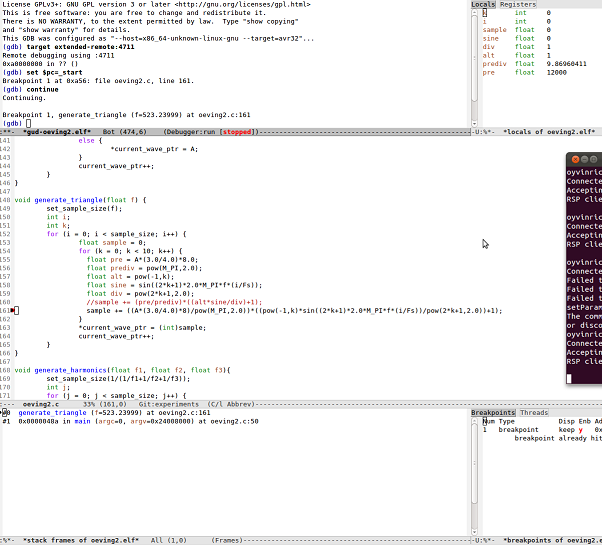
\includegraphics{images/debugsmall.png}
Figure 2: Debugging the \emph{generateTriangle} function
\end{center}

\section{Results}
\subsection{Description} 

This exercise resulted in a working sokoban game on the STK1000 development board displayed. The game is played by using the buttons as controllers to move around in the game which is displayed on the LCD screen. In addition to a general "arrow key" setup, there is also a possibility to undo and redo with the buttons. 

\subsection{Feedback}There are sounds and LEDs to help you understand the game play better through audiovisual feedback. The LEDs show how many crates you have left in the game, and when you win all LEDs will blink several times to emphasize your epic win.

\subsection{Sounds}There are sounds for the start of the game, when you place a crate on a target, when you remove a crate from a target, when you hit a wall and when you win. When you win there will also be a splash screen telling you that you've won. 

\subsection{Game play}
In regards to the game play we have movement in four directions, the ability to push crates, disability to walk through walls, and the ability to undo and redo. 

\subsection{Technical aspects}Technically the resulting game is written in C code on top of a linux operating system. To manage the LEDs and buttons we have written two corresponding linux drivers that operates as interfaces between the STK1000 development board and linux. 


\section{Tests}
\subsection{Description}

We've created a few test scenarios in order to test different aspects of our game functionality. The tests were conducted by a person interacting with the switches and looking at the LCD screen, wearing a headset. Another person logged the results of the test. The main equipment was the STK1000 development board and a headset with the main focus on the LCD screen. The jumpers of the board were set as specified in the compendium (section 4.2) \cite{komp}. The GPIO was set up with both LEDs and switches connected to B as follows: LEDs on 8-15, switches on 0-7. 





\subsection{Results}
Below is a table of the different tests we ran, the preconditions and the results. 


\begin{center}
\footnotesize
\renewcommand{\arraystretch}{1.25} %vertical cell padding
\begin{tabular}[pos]{|m{45pt}|m{80pt}|m{90pt}|m{105pt}|m{60pt}|}
\hline  \textbf{Name} & \textbf{Description} & \textbf{Conditions} & \textbf{Expected} & \textbf{Results} \\ 

\hline Steady-state test & Power is on and the main program is running & The board has been programmed and powered on & The board is powered and no LEDs or sounds should be on & Passed \\

\hline Left & Player is moved left & A level is loaded and there is free space to the left of the player & Player moves to the left when \emph{SW7} is pressed.  & Passed \\

\hline Down & Player is moved down & A level is loaded and there is free space beneath the player & Player moves down when \emph{SW6} is pressed.  & Passed \\

\hline Up & Player is moved up & A level is loaded and there is free space above the player & Player moves up when \emph{SW5} is pressed.  & Passed \\

\hline Right & Player is moved right & A level is loaded and there is free space to the right of the player & Player moves to the right when \emph{SW4} is pressed.  & Passed \\

\hline Undo & The last move is undone & At least one move is made & The last move is undone when \emph{SW3} is pressed.  & Passed \\

\hline Redo & The last undo is undone & Undo must have been done as the previous move. & The undone move is redone when \emph{SW2} is pressed.  & Passed \\

\hline Reset level & The loaded level is reset & A level must have been loaded and the game may or may not have been initialized & Level is reset when \emph{SW1} is pressed.  & Passed \\

\hline Return to main menu & Main menu is displayed & Sokoban is loaded?? & Main menu is displayed when \emph{SW0} is pressed.  & Passed \\


\hline 
\end{tabular} 
\end{center}

\newpage

\section{Evaluation of assignment}

We found it interesting to learn more about the inner workings of linux and how a device driver is written. 

We had quite a lot of problems with getting linux to work. This was much due to the guide we got didn't really seem to work, at least no one that we talked to made it work through following that guide. Another group posted a different guide that we managed to get working. But in general this wasted much time for us and should be improved. 

\section{Conclusion}
%We learned how to generate and play different sounds in C. This will be helpful when we start coding the next assignment. In the end we have four different sounds. Three short sound effects and one melody. 

\footnotesize{  % This makes the Reference items print in footnotesize fonts
\begin{thebibliography}{N}

\bibitem[1]{avrdoc} AVR32 Architecture Document
\url{http://www.atmel.com/images/doc32000.pdf}

\bibitem[2]{stkdoc} AT32AP7000 Datasheet
\url{http://www.atmel.com/Images/doc32003.pdf}

\bibitem[3]{komp} TDT4258 Compendium
\url{http://www.idi.ntnu.no/emner/tdt4258/_media/kompendium.pdf}

\bibitem[4]{sokoban} Description of the game Sokoban on Sokoban Wiki . Retrieved 23.04.13.
\url{http://www.sokobano.de/wiki/index.php?title=The_rules_of_the_game}

\bibitem[5]{sokobanlevel} Description of Sokobon levels on Sokoban Wiki. Retrieved 23.04.13.
\url{http://www.sokobano.de/wiki/index.php?title=Level_format}

\bibitem[5]{sokobanscreen} Screenshot based on Sokoban skins on GitHub. Retrieved 23.04.13.
\url{https://github.com/borgar/sokoban-skins}


\end{thebibliography}  
}

\end{document} 
